


\begin{applicationActivities}

\begin{definition}
A \term{linear transformation} is a map between vector spaces that preserves the vector space operations.  More precisely, if $V$ and $W$ are vector spaces, a map $T:V\rightarrow W$ is called a linear transformation if
\begin{enumerate}
\item $T(\vec{v}+\vec{w}) = T(\vec{v})+T(\vec{w})$ for any $\vec{v},\vec{w} \in V$
\item $T(c\vec{v}) = cT(\vec{v})$ for any $c \in \IR$, $\vec{v} \in V$.
\end{enumerate}
In other words, a map is linear if one can do vector space operations before applying the map or after, and obtain the same answer.
\end{definition}

\begin{definition}
Given a linear transformation \(T:V\to W\),
$V$ is called the \term{domain} of $T$ and
$W$ is called the \term{co-domain} of $T$.

\begin{center}
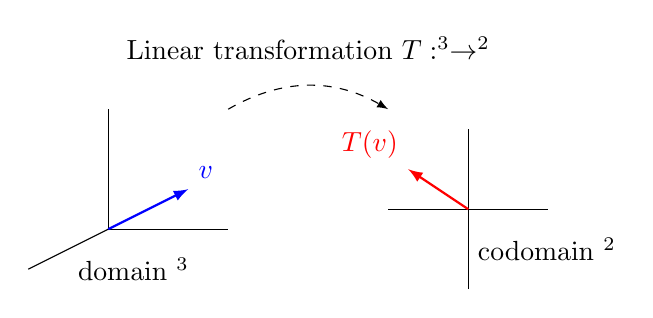
\begin{tikzpicture}[x=0.2in,y=0.2in]
  \begin{scope}[shift={(0,0)}]
    \draw (0,0) -- (3,0);
    \draw (0,0) -- (0,3);
    \draw (0,0) -- (-2,-1);
    \draw[thick,-latex,blue] (0,0) -- (2,1)
          node[anchor=south west] {\(\vect v\)};
    \node[anchor=west] at (-1,-1) {domain \(\IR^3\)};
  \end{scope}
  \draw[dashed,-latex] (3,3) to [bend left=30] (7,3);
  \node[anchor=south] at (5,4) {Linear transformation \(T:\IR^3\to\IR^2\)};
  \begin{scope}[shift={(9,0.5)}]
    \draw (-2,0) -- (2,0);
    \draw (0,-2) -- (0,2);
    \draw[thick,-latex,red] (0,0) -- (-1.5,1)
          node[anchor=south east] {\(T(\vect v)\)};
    \node[anchor=west] at (0,-1) {codomain \(\IR^2\)};
  \end{scope}
\end{tikzpicture}
\end{center}
\end{definition}

\begin{example}
Let $T : \IR^3 \rightarrow \IR^2$ be given by $$T\left(\begin{bmatrix} x \\ y \\ z \end{bmatrix} \right) = \begin{bmatrix} x-z \\ y \end{bmatrix}$$

To show that \(T\) is linear, we must verify...
\[
  T\left(
    \begin{bmatrix} x_1 \\ y_1 \\ z_1 \end{bmatrix} +
    \begin{bmatrix}x_2 \\ y_2  \\ z_2 \end{bmatrix}
  \right)
=
  T\left(
    \begin{bmatrix} x_1+x_2 \\ y_1+y_2 \\ z_1+z_2 \end{bmatrix}
  \right) =
  \begin{bmatrix} (x_1+x_2)-(z_1+z_2) \\ (y_1+y_2) \end{bmatrix}
\]
\[
  T\left(
    \begin{bmatrix} x_1 \\ y_1 \\ z_1 \end{bmatrix}
  \right) + T\left(
    \begin{bmatrix} x_2 \\ y_2 \\ z_2 \end{bmatrix}
  \right)
=
  \begin{bmatrix} x_1-z_1 \\ y_1 \end{bmatrix} +
  \begin{bmatrix} x_2-z_2 \\ y_2 \end{bmatrix}=
  \begin{bmatrix} (x_1+x_2)-(z_1+z_2) \\ (y_1+y_2) \end{bmatrix}
\]
And also...
\[
  T\left(c\begin{bmatrix} x \\ y \\ z \end{bmatrix} \right)
=
  T\left(\begin{bmatrix} cx \\ cy \\ cz \end{bmatrix} \right)
=
  \begin{bmatrix} cx-cz \\ cy \end{bmatrix}
\text{ and }
  cT\left(\begin{bmatrix} x \\ y \\ z \end{bmatrix} \right)
=
  c\begin{bmatrix} x-z \\ y \end{bmatrix}
=
  \begin{bmatrix} cx-cz \\ cy \end{bmatrix}
\]

Therefore $T$ is a linear transformation.
\end{example}


\begin{activity}{15}
Determine if each of the following maps are linear transformations
\begin{subactivity}
$T_1: \IR^2 \rightarrow \IR$ given by $T_1 \left(\begin{bmatrix} x \\ y \end{bmatrix} \right) = \sqrt{x^2+y^2}$.
\end{subactivity}
\begin{subactivity}
$T_2: \IR^3 \rightarrow \IR^3 $ given by $T_2\left(\begin{bmatrix} x \\ y \\ z \end{bmatrix} \right)  = \begin{bmatrix} -x \\ -y \\ -z \end{bmatrix}$
\end{subactivity}
\begin{subactivity}
$T_3: \P^d \rightarrow \P^{d-1}$ given by $T_3(f(x)) = f^\prime(x)$.
\end{subactivity}
\begin{subactivity}
$T_4: \P \rightarrow \P$ given by $T_4(f(x)) = f(x)+x^2$
\end{subactivity}
\end{activity}

\begin{activity}{5}
Suppose $T: \IR^3 \rightarrow \IR^2$ is a linear transformation, and you know $T\left(\begin{bmatrix} 1 \\ 0 \\ 0 \end{bmatrix} \right) = \begin{bmatrix} 2 \\ 1 \end{bmatrix} $ and $T\left(\begin{bmatrix} 0 \\ 0 \\ 1 \end{bmatrix} \right) = \begin{bmatrix} -3 \\ 2 \end{bmatrix} $.  Compute $T\left(\begin{bmatrix} 3 \\ 0 \\ 0 \end{bmatrix}\right)$.
\begin{multicols}{2}
\begin{enumerate}[(a)]
\item $\begin{bmatrix} 6 \\ 3\end{bmatrix}$
\item $\begin{bmatrix} -9 \\ 6 \end{bmatrix}$
\item $\begin{bmatrix} -4 \\ -2 \end{bmatrix}$
\item $\begin{bmatrix} 6 \\ -4 \end{bmatrix}$
\end{enumerate}
\end{multicols}
\end{activity}

\begin{activity}{3}
Suppose $T: \IR^3 \rightarrow \IR^2$ is a linear transformation, and you know $T\left(\begin{bmatrix} 1 \\ 0 \\ 0 \end{bmatrix} \right) = \begin{bmatrix} 2 \\ 1 \end{bmatrix} $ and $T\left(\begin{bmatrix} 0 \\ 0 \\ 1 \end{bmatrix} \right) = \begin{bmatrix} -3 \\ 2 \end{bmatrix} $.  Compute $T\left(\begin{bmatrix} 0 \\ 0 \\ -2 \end{bmatrix}\right)$.
\begin{multicols}{2}
\begin{enumerate}[(a)]
\item $\begin{bmatrix} 6 \\ 3\end{bmatrix}$
\item $\begin{bmatrix} -9 \\ 6 \end{bmatrix}$
\item $\begin{bmatrix} -4 \\ -2 \end{bmatrix}$
\item $\begin{bmatrix} 6 \\ -4 \end{bmatrix}$
\end{enumerate}
\end{multicols}
\end{activity}

\begin{activity}{5}
Suppose $T: \IR^3 \rightarrow \IR^2$ is a linear transformation, and you know $T\left(\begin{bmatrix} 1 \\ 0 \\ 0 \end{bmatrix} \right) = \begin{bmatrix} 2 \\ 1 \end{bmatrix} $ and $T\left(\begin{bmatrix} 0 \\ 0 \\ 1 \end{bmatrix} \right) = \begin{bmatrix} -3 \\ 2 \end{bmatrix} $.  Compute $T\left(\begin{bmatrix} 1 \\ 0 \\ 1 \end{bmatrix}\right)$.
\begin{multicols}{2}
\begin{enumerate}[(a)]
\item $\begin{bmatrix} 2 \\ 1\end{bmatrix}$
\item $\begin{bmatrix} 3 \\ -1 \end{bmatrix}$
\item $\begin{bmatrix} -1 \\ 3 \end{bmatrix}$
\item $\begin{bmatrix} 5 \\ -8 \end{bmatrix}$
\end{enumerate}
\end{multicols}
\end{activity}

\begin{activity}{2}
Suppose $T: \IR^3 \rightarrow \IR^2$ is a linear transformation, and you know $T\left(\begin{bmatrix} 1 \\ 0 \\ 0 \end{bmatrix} \right) = \begin{bmatrix} 2 \\ 1 \end{bmatrix} $ and $T\left(\begin{bmatrix} 0 \\ 0 \\ 1 \end{bmatrix} \right) = \begin{bmatrix} -3 \\ 2 \end{bmatrix} $.  Compute $T\left(\begin{bmatrix} -2 \\ 0 \\ -3 \end{bmatrix}\right)$.
\begin{multicols}{2}
\begin{enumerate}[(a)]
\item $\begin{bmatrix} 2 \\ 1\end{bmatrix}$
\item $\begin{bmatrix} 3 \\ -1 \end{bmatrix}$
\item $\begin{bmatrix} -1 \\ 3 \end{bmatrix}$
\item $\begin{bmatrix} 5 \\ -8 \end{bmatrix}$
\end{enumerate}
\end{multicols}
\end{activity}

\begin{activity}{5}
Suppose $T: \IR^4 \rightarrow \IR^3$ is a linear transformation.
How many facts of the form $T(\vec{v}_i)=\vec{w}_i$ do you need to know in order to be able to compute $T(\vec{v})$ for \textit{any} $\vec{v} \in \IR^4$?
\begin{enumerate}[(a)]
\item $2$
\item $3$
\item $4$
\item $5$
\item You need infinitely many
\end{enumerate}
(In this situation, we say that the vectors \(\{\vect v_1,\dots,\vect v_n\}\)
\term{determine} \(T\).)
\end{activity}

\begin{fact}
Consider any basis \(\{\vect b_1,\dots,\vect b_n\}\) for $V$.  Since every vector can be written \textit{uniquely} as a linear combination of basis vectors, every linear transformation $T:V \rightarrow W$ is determined by those basis vectors.

\[
  T(\vect v)=T(x_1\vect b_1+\dots+ x_n\vect b_n)=
  x_1T(\vect b_1)+\dots+x_nT(\vect b_n)
\]
\end{fact}

\begin{definition}
The \term{standard basis} of $\IR^n$ is the (ordered) basis $\{\vec{e}_1, \vec{e}_2, \ldots, \vec{e}_n\}$ where
\begin{align*}
\vec{e}_1 &= \begin{bmatrix} 1 \\ 0 \\ 0 \\\vdots \\ 0 \\ 0 \end{bmatrix}  &
\vec{e}_2 &= \begin{bmatrix} 0 \\ 1 \\ 0 \\\vdots \\ 0 \\ 0 \end{bmatrix}  & \cdots  & &
\vec{e}_n &= \begin{bmatrix} 0 \\ 0 \\ 0 \\\vdots \\ 0 \\ 1 \end{bmatrix}
\end{align*}

Since linear transformation \(T:\IR^n\to\IR^m\) is determined by
the values of each \(T(\vec e_i)\), it's convenient to store this
information in the \(m\times n\) \term{standard matrix}
\([T(\vec e_1) \,\cdots\, T(\vect e_n)]\).
\end{definition}


\begin{example}
Let $T: \IR^3 \rightarrow \IR^2$ be the linear transformation determined by
the following values for \(T\) applied to the standard basis of \(\IR^3\).
\begin{align*}
T\left(\begin{bmatrix} 1 \\ 0 \\ 0 \end{bmatrix} \right) &= \begin{bmatrix} 3 \\ 2\end{bmatrix} &
T\left(\begin{bmatrix} 0 \\ 1 \\ 0 \end{bmatrix} \right) &= \begin{bmatrix} -1 \\ 4\end{bmatrix} &
T\left(\begin{bmatrix} 0 \\ 0 \\ 1 \end{bmatrix} \right) &= \begin{bmatrix} 5 \\ 0\end{bmatrix}
\end{align*}

Then the standard matrix corresponding to $T$
is $$\begin{bmatrix}3 & -1 & 5 \\ 2 & 4 & 0 \end{bmatrix}.$$
\end{example}

\begin{activity}{5}
  Let $T: \IR^3 \rightarrow \IR^2$ be the linear transformation given by
$$T\left(\begin{bmatrix} x\\ y \\ z \end{bmatrix} \right) = \begin{bmatrix} x+3z \\ 2x-y-4z \end{bmatrix}$$
Write the matrix corresponding to this linear transformation with respect to the standard basis.
\end{activity}

\begin{activity}{5}
  Let $T: \IR^3 \rightarrow \IR^2$ be the linear transformation given by the standard matrix $$\begin{bmatrix} 3  & -2 & -1  \\ 4 & 5 & 2 \end{bmatrix}.$$

Compute $T\left(\begin{bmatrix} x\\ y \\ z \end{bmatrix} \right) $.
\end{activity}

% \begin{fact}
%   $T: \IR^n \rightarrow \IR^m$ is given by the matrix
%   \([\vect v_1 \,\cdots\, \vect v_n]\) exactly when
%   \(T\left(
%     \begin{bmatrix}
%       x_1 \\ \vdots \\ x_n
%     \end{bmatrix}
%   \right)
%     =
%   x_1\vect v_1 + \dots + x_n\vect v_n\).
% \end{fact}

\begin{activity}{10}
Let $D: \P^3 \rightarrow \P^2$ be the derivative map \(D(f(x))=f'(x)\).
(Earlier we showed this is a linear transformation.)
\begin{subactivity}
Write down an equivalent linear transformation $T: \IR^4 \rightarrow \IR^3$
by converting \(\{1,x,x^2,x^3\}\) and \(\{D(1),D(x),D(x^2),D(x^3)\}\) into
appropriate vectors in \(\IR^4\) and \(\IR^3\).
\end{subactivity}
\begin{subactivity}
Write the standard matrix corresponding to $T$.
\end{subactivity}
\end{activity}

\end{applicationActivities}
